\section{The Paṇḍaka}

\subsection{The Paṇḍaka in the Pali Vinaya}
In the \textit{Theravāda Vinaya} the term \textit{paṇḍaka} is mainly used in the context of individuals a monastic should not have sexual relations with or as a form of insult. The rule regarding the ordination of \textit{paṇḍakas} is laid down in \textit{Khandhaka} 1\footnote{\textit{Khandhaka} 1 \textit{Pabbajjā} PTS vol 1 pages 85–86.} and reads as follows:\footnote{Translation by Ajahn Brahmali.}

\begin{quote}
\textit{Tena kho pana samayena aññataro paṇḍako bhikkhūsu pabbajito hoti. So dahare dahare bhikkhū upasaṅkamitvā evaṁ vadeti—``etha, maṁ āyasmanto dūsethā''ti. Bhikkhū apasādenti—``nassa, paṇḍaka, vinassa, paṇḍaka, ko tayā attho''ti. So bhikkhūhi apasādito mahante mahante moḷigalle sāmaṇere upasaṅkamitvā evaṁ vadeti—``etha, maṁ āvuso dūsethā''ti. Sāmaṇerā apasādenti—``nassa, paṇḍaka, vinassa, paṇḍaka, ko tayā attho''ti. So sāmaṇerehi apasādito hatthibhaṇḍe assabhaṇḍe upasaṅkamitvā evaṁ vadeti—``etha, maṁ āvuso dūsethā''ti. Hatthibhaṇḍā assabhaṇḍā dūsesuṁ. Te ujjhāyanti khiyyanti vipācenti—``paṇḍakā ime samaṇā sakyaputtiyā. Yepi imesaṁ na paṇḍakā, tepi ime paṇḍake dūsenti. Evaṁ ime sabbeva abrahmacārino''ti. Assosuṁ kho bhikkhū tesaṁ hatthibhaṇḍānaṁ assabhaṇḍānaṁ ujjhāyantānaṁ khiyyantānaṁ vipācentānaṁ. Atha kho te bhikkhū bhagavato etamatthaṁ ārocesuṁ. ``Paṇḍako, bhikkhave, anupasampanno na upasampādetabbo, upasampanno nāsetabbo''ti.}
\end{quote}

\begin{quote}
At one time a certain \textit{paṇḍaka} had gone forth as a monk. He approached the young monks and said, ``Venerables, come and have sex with me.'' The monks dismissed him, ``Go away, \textit{paṇḍaka}. Who wants you?''

He went to the big and fat novices, said the same thing, and got the same response.

He then went to the elephant keepers and horse keepers, and once again he said the same thing. And they had sex with him. They complained and criticized them, ``These Sakyan ascetics are \textit{paṇḍakas}. And those who are not have sex with them. None of them is celibate.''

The monks heard their complaints. They told the Buddha and he said, ``A \textit{paṇḍaka} should not be given the full ordination. If it has been given, he should be expelled.''
\end{quote}

There are a couple of interesting things to note about this passage. First of all, the \textit{paṇḍaka} in question was already ordained at the time of this incident. The rule against ordination of \textit{paṇḍakas} clearly mentions that full ordination of these individuals, the \textit{upasampadā}, is not allowed. This really only makes sense if we understand the word \textit{pabbajjā} (translated by Ajahn Brahmali as `gone forth') here to be equivalent to \textit{upasampadā}. In fact this equivalence between \textit{pabbajjā} and \textit{upasampadā} is what we find throughout the earliest \textit{Vinaya}, and indeed the \textit{Suttas}.\footnote{The \textit{sāmaṇeras/īs} are barely mentioned in the \textit{Suttas}. Instead we find the figure of the \textit{samaṇuddesa}, `one designated as a \textit{samaṇa}', who seems to have had a looser affiliation with the \textit{Saṅgha}, that is, no proper ordination. The commentaries gloss them as \textit{sāmaṇeras}, but this might be an oversimplification. More likely they were a kind of precursor to the more formal status of novice. It seems likely that such people merely put on robes, and then lived with a loose connection to a particular community of ascetics, in which case their sex and gender would have been a non-issue. I would argue it is natural to see novices proper in the same way. But the \textit{samaṇuddesa} remains obscure.} In any case, the rule itself is clearly limited to \textit{upasampadā} (full ordination) and novice ordination seems to be allowed.

The \textit{Theravāda} commentary, both in regards to the \textit{paṇḍaka} and the \textit{ubhatob­yañ­janaka}, differs from the \textit{Vinaya} in making a distinction between \textit{pabbajjā} (in the meaning of novice ordination) and \textit{upasampadā} (full ordination) and does not allow either.

We would expect that the \textit{paṇḍaka} (and the same counts for the \textit{ubhatob­yañ­janaka}) in this story would be expelled from the Order on the grounds of breaking the first rule of conduct in the \textit{pāṭimokkha}, namely the rule against sexual intercourse (\textit{pārājika} 1\footnote{PTS vol. 3 page 1.}). This is the very first rule that was laid down by the Buddha. Instead, not only is he expelled but also all others who are judged to be a \textit{paṇḍaka}, even if those others were examplary monks themselves. Brenna Artinger\footnote{\cite{artinger} page 21.} points out that there seems to be the perception (or prejudice) of a fundamental mental flaw in \textit{paṇḍakas} that makes them especially troublesome and unable to remain celibate. The promiscuous nature of the \textit{paṇḍaka} would harm the whole \textit{Saṅgha} and give it a bad name among the lay supporters on which it depends.

Another interesting point is that the monks and novices that are approached by the \textit{paṇḍaka} react in an exemplary manner and send him away. It is only the elephant and horse keepers, those of a lower class, who engage in sexual relations with him. But afterwards, they still complain about it and criticize the \textit{paṇḍaka} while they have themselves also engaged in the same act. This seems a bit odd and revolves around the stock passage ``\textit{Te ujjhāyanti khiyyanti vipācenti}'' (``They complained and criticized them'') that is used throughout the \textit{Vinaya} as a typical pattern of narration. In the majority of cases it is the \textit{manussā} (people) who complain and criticize, after which the monks would hear about it, also complain and criticize (``\textit{Ye te bhikkhū appicchā …pe… te ujjhāyanti khiyyanti vipācenti}'') and then relate the story to the Buddha. So the word \textit{te} (they) usually refers to the monks who criticize after they have heard it from the `people'. Here however the word \textit{te} is used right after the elephant and horse keepers, seemingly referring to them. However, it would make much more sense if others would complain about this scandalous behavior rather than the elephant and horse keepers themselves. Indeed this is what we find in the same story in the \textit{Dharmaguptaka} \textit{Vinaya}, where the people (lay Buddhists) complain and criticize (時諸居士見已譏嫌言). Claire Maes\footnote{\cite{maes2011} pages 98–101.} points out that this phrase could have been used to conceal debates that might have influenced the \textit{Bhikkhu Saṅgha} to implement specific precepts to be in conformity with the praxes of other ascetic communities with the main purpose of placing the origin of precepts within the Buddhist Order with the Buddha himself in a leading role. She successfully demonstrates this with the Jain concept of \textit{ekindriya jīva} (one-facultied life) and argues that this concept entered the Buddhist \textit{Vinaya} as a result of interactions and discussions with the Jain contemporaries. I believe that the term \textit{paṇḍaka} could also have entered the Buddhist \textit{Vinaya} in a similar manner. As we have seen previously, the position of the \textit{paṇḍaka} was discussed at length in the debate among the Jains.

In Appendix \ref{appendix2}, Section \ref{appendix2a}, I have charted the occurrences of the various words throughout the texts. This illustrates that the term \textit{paṇḍaka} mainly occurs in the \textit{Vinaya} and the commentaries of the Pali texts and is relatively most important in the \textit{Vinaya}. The Sanskrit texts are not entirely organized by lateness but it is clear that the term \textit{paṇḍaka} mainly appears in the \textit{Vinaya} and \textit{Śāstrapiṭaka}. The term \textit{klība} is notable by its absence in all Buddhist texts and only appears in the Vedic and later Brahmanical texts. One explanation for this might be that the terms \textit{klība} and \textit{paṇḍaka} have been mixed up because their meanings were at least in part overlapping. What is also striking is that the umbrella term \textit{napuṁsaka} only appears in the Pali commentarial texts and not in any of the earlier collections. It is however a recurrent term in the Vedic and Brahmanical texts. We also see that this term becomes more prominent in the later Anya commentaries as well as in the Brahmanical \textit{Śāstra} collections, which points to a shift in emphasis, and possibly meaning, of this term in later times at the expense of the prominence of the term \textit{paṇḍaka}. As these are later texts I have not looked into them in great detail and this might be an interesting topic for future studies.

Considering that the word \textit{paṇḍaka} does not appear in any of the early \textit{Suttas}, nor in the early parts of the \textit{Vinaya},\footnote{The word is not found in the \textit{pātimokkhas}, the lists of rules for monastics. Next to the Pali \textit{Vinaya}, it appears twice in the \textit{Aṅguttara Nikāya}, but both of these occurrences only have parallels to the \textit{Vinaya} or later texts and are most likely later additions.} this is an indication that the inclusion of the word in the \textit{Vinaya} did not happen in the Buddha's lifetime but was added later as a result of the discussions with the Brahmins and Jains, for whom \textit{paṇḍakas} could not ordain.

Brenna Artinger\footnote{\cite{artinger} pages 26–32} discusses the idea found in commentarial and \textit{Abhidhamma} texts that \textit{paṇḍakas}, \textit{ṣaṇḍhas} and \textit{ubhatob­yañ­janakas} are unable to practice the Dhamma because due to their inherent \textit{kamma} they do not have the capacity for cultivation of any kind. They mention that they finds the lack of examples of \textit{paṇḍaka} and other sexual nonconforming individuals in these texts problematic and there is a lack of data from which these statements can be made. It seems to me a highly theoretical stance and it could indeed be the reason why the rule prohibiting \textit{paṇḍakas} and the \textit{ubhatob­yañ­janakas} from ordaining was included in the \textit{Vinaya}. This would be another indication of the later origins of this clause. In his analysis of the \textit{Bhikkhunī} \textit{Vinaya} Bhikkhu Sujato\footnote{\cite{sujato2009} pages 211–216.} points out that there is indeed a strong relationship between the \textit{Vinaya} and the later \textit{Abhidhamma} texts.

\subsection{The Five Types of Paṇḍaka}
Going beyond the \textit{Vinaya} itself into the commentarial scriptures, we find the following explanation in the \textit{Theravāda} \textit{Samantapāsādikā} with regards to the nature of the \textit{paṇḍaka}:\footnote{\textit{Samantapāsādikā}: Vol. V, p. 1015f. Translations/explanations as in \cite{bomhard}, \cite{thanissaro} and \cite{artinger} pages 22–23.}

\begin{quote}
\textit{Paṇḍakobhikkhaveti ettha āsittapaṇḍako usūyapaṇḍako opakkamikapaṇḍako pakkhapaṇḍako napuṁsakapaṇḍakoti pañca paṇḍakā. Tattha yassa paresaṁ aṅgajātaṁ mukhena gahetvā asucinā āsittassa pariḷāho vūpasammati, ayaṁ āsittapaṇḍako. Yassa paresaṁ ajjhācāraṁ passato usūyāya uppannāya pariḷāho vūpasammati, ayaṁ usūyapaṇḍako. Yassa upakkamena bījāni apanītāni, ayaṁ opakkamikapaṇḍako. Ekacco pana akusalavipākānubhāvena kāḷapakkhe paṇḍako hoti, juṇhapakkhe panassa pariḷāho vūpasammati, ayaṁ pakkhapaṇḍako. Yo pana paṭisandhiyaṁyeva abhāvako uppanno, ayaṁ napuṁsakapaṇḍakoti. Tesu āsittapaṇḍakassa ca usūyapaṇḍakassa ca pabbajjā na vāritā, itaresaṁ tiṇṇaṁ vāritā. Tesupi pakkhapaṇḍakassa yasmiṁ pakkhe paṇḍako hoti, tasmiṁyevassa pakkhe pabbajjā vāritāti kurundiyaṁ vuttaṁ. Yassa cettha pabbajjā vāritā, taṁ sandhāya idaṁ vuttaṁ--``anupasampanno na upasampādetabbo upasampanno nāsetabbo''ti. Sopi liṅganāsaneneva nāsetabbo. Ito paraṁ ``nāsetabbo''ti vuttesupi eseva nayo.}
\end{quote}

\begin{quote}
A `\textit{paṇḍaka}', monks, means in this case, \textit{āsittapaṇḍaka}, \textit{usūyapaṇḍaka}, \textit{opakkamikapaṇḍaka}, \textit{pakkhapaṇḍaka}, \textit{napuṁsakapaṇḍaka}. Five \textit{paṇḍakas}:

\begin{enumerate}
\item \textit{āsittapaṇḍaka}: a man who gains satisfaction from performing oral sex on another man and from swallowing his semen or who only becomes sexually aroused after swallowing another man's semen. 
\item \textit{usūyapaṇḍaka}: a voyeur, that is, a person who gains sexual satisfaction from watching others have sex. 
\item \textit{opakkamikapaṇḍaka}: eunuch, due to castration.
\item \textit{pakkhapaṇḍaka}: those who become sexually aroused in parallel with the phases of the moon.\footnote{According to \cite{bomhard}, the term \textit{pakkhapaṇḍaka} (Skt. \textit{pakṣapaṇḍaka}) probably does not refer, as traditionally understood, to an individual who becomes sexually aroused parallel to the phases of the moon, i.e., to someone who is aroused during the fortnight of either the waxing or waning moon, but to someone ``who acts wrongly sexually, who behaves badly sexually.'' He hypothesizes that \textit{pakkha} of the compound \textit{pakkhapaṇḍaka} should be understood in terms of its alternative meaning `a cripple', and that the corresponding Sanskrit should not be understood as \textit{pakṣa} but rather \textit{phakka} (`cripple', adj. `lame, crippled, maimed'), derived from the Skt. verbal root \textit{phakk}, ``(a) to creep, to steal along; (b) to have a preconceived opinion; (c) to act wrongly, to behave badly.'' He thus considers the third meaning of \textit{phakk} as most relevant to the case at hand.}
\item \textit{napuṁsakapaṇḍaka}: a person born without sexual organs.\footnote{The Sanskrit equivalent is \textit{prakṛtipaṇḍaka}. The term \textit{prakṛti} means something like `nature' or `fundamental form' and the term \textit{tṛtīyāprakṛti} became the official word for the `third sex' at around the beginning of the Common Era. I therefore do not believe this translation by \cite{thanissaro} to be correct but that the literal meaning reflects more the original meaning of \textit{napuṁsaka}.} 
\end{enumerate}

Of these, the \textit{āsittapaṇḍaka} and \textit{usūyapaṇḍaka} are not prevented from ordination, but the other three are prevented. It is said in the \textit{Kurundi} [commentary], ``of these, the \textit{pakkhapaṇḍaka} is prevented from ordination in the fortnight in which they are a \textit{paṇḍaka}.'' In this case with regards to those who are prevented from ordination, it is said, ``if they are ordained they should be expelled.'' He should be expelled just by confiscation of his robe. Hereafter, when it is said that ``he should be expelled'', this is the procedure.
\end{quote}

The castrated \textit{paṇḍaka} i.e. a eunuch, is only one of the three types that cannot ordain, which makes it highly unlikely that the word \textit{paṇḍaka} means `eunuch', at least at the time these five types were defined. We would also not expect a eunuch to have hyperlibidinous-ness. After all, castrated men were often employed as harem guards just for the reason that they are no longer interested in sexual activity and therefore considered safe. Moreover, the \textit{Dharmaguptaka} \textit{Vinaya} treats the castrated man as something other than a \textit{paṇḍaka}. However, as we have seen in Tantric Hinduism these men had a social religious function that involved the provision of alternative sexual techniques according to the sacred texts, at least from the middle of the 1\textsuperscript{st} millennium CE or thereafter.

As we have seen in the Jain scriptures, the discussion to overcome the ambiguities in the understanding of the word \textit{napuṁsaka} resulted over time in changes in meaning and the definition of sub-categories, and I believe this has also occurred in the Buddhist \textit{Vinayas} with the word \textit{paṇḍaka}. I believe that it is likely that the term \textit{opakkamikapaṇḍaka} represented a castrated man, the \textit{klība}, while the \textit{napuṁsakapaṇḍaka} was the re-definition of the original \textit{paṇḍaka} or the `female \textit{napuṁsaka}' that we saw emerging in the Jain commentarial texts. Also from the Chinese sources it is clear that the person has to be born this way.

The \textit{pakkhapaṇḍaka} is interesting and several explanations have been given by authors over time, none of which I find convincing. Allan \cite{bomhard} advocates that the word \textit{pakkha} should not be translated as `half moon' but that the meaning of the word is something like a sex-addict. I refute this argument because the characters used to denote this type of \textit{paṇḍaka} in the Chinese \textit{Vinayas} of all schools are 半月, which literally means `half moon'. It is also mentioned in various Chinese commentarial texts\footnote{f.i. X44 0744 0432c17 四分律名義標釋.} that the `half moon' is `not a male' and thus a form of \textit{napuṁsaka} for half of the month and the other half he is a male. All texts are consistent in this. As we can still understand the meaning of the other four categories in light of people's physiology or sexual fetishes, the `half-moon' \textit{paṇḍaka} is an enigma. Turning back to the Vedic texts however, we find in the \textit{Uttarakanda} of the \textit{Rāmāyaṇam}\footnote{Rām 7.78–79. See also \cite{goldman} pages 379–380.} the story of King Ila. In this epic tale the king accidentally stumbles upon the Goddess Pārvatī in intimate embrace with Śiva, who turns him into a woman. Now Ilā, she turns to the Goddess for mercy to restore her manhood but is only granted half her wish, namely that she has to change sex/gender each month. The theme of changing sex and gender based on the phases of the moon is a recurrent theme in the Vedic myths and it is not unlikely that this mythical theme has found its way into the commentaries in the form of the \textit{pakkhapaṇḍaka}. After all, another rule in the \textit{Vinayas} of all the schools tells the tale of a shape-shifting serpent, a mythological beast, a \textit{Nāga},\footnote{\textit{Khandhaka} 1 \textit{Pabbajjā} PTS vol 1 pages 86–88.} who ordains as a monk, is later discovered and a new rule is laid down in much the same manner as for the \textit{paṇḍaka}, barring him and all his kind from ordination. The fabric of myth and reality can easily overlap in Indic culture. The \textit{Vinaya} is full of various strange and wonderful beings. The ­\textit{Bhikkhu Pā­rāji­ka} 1, the rule against sexual intercourse, mentions that a monk is not allowed to have sex with a list of beings, namely a dragon, a spirit, a ghost and a \textit{paṇḍaka}.\footnote{PTS vol. 3 page 37: \textit{Tena kho pana samayena aññataro bhikkhu nāgiyā methunaṁ dhammaṁ paṭisevi … yakkhiniyā methunaṁ dhammaṁ paṭisevi … petiyā methunaṁ dhammaṁ paṭisevi … paṇḍakassa methunaṁ dhammaṁ paṭisevi. Tassa kukkuccaṁ ahosi … pe … ``āpattiṁ tvaṁ, bhikkhu, āpanno pārājikan''ti.}} The fact that the \textit{paṇḍaka} is listed in a list of mythological beings is indicative of its origins and how they were viewed at that time. We find similar lists in the \textit{Vinayas} of the other schools.

As for the other two types of \textit{paṇḍaka}, the \textit{āsittapaṇḍaka} and the \textit{usūyapaṇḍaka}, who at least in the \textit{Theravāda} tradition are allowed to ordain, I believe they embody another of the Jain categories, namely the category of the \textit{puruṣanapuṁsaka} (male \textit{napuṁsaka}). Although they might be impotent and are therefore also in possession of the female \textit{veda}, their appearance is male to the lay supporters but also to the celibate monks they live with who are not aroused by their presence. The relaxation of the rules for these two types also runs parallel with the development in the Jain scriptures. But unlike the Jains, no further abolishment of this entire rule against the ordination of \textit{paṇḍakas} was reached simply because the Buddhist scriptures were closed while the Jain scriptures continued to evolve for many centuries thereafter.

One consistent characteristic of the \textit{paṇḍaka} which we find throughout the \textit{Vinayas} of all the schools is that they are perceived as troublesome as a monastic because they are unable to maintain their precept of celibacy due to their hyperlibidinous nature. However, the \textit{āsittapaṇḍaka} and the \textit{usūyapaṇḍaka} are, judging from their description, far more sexually active than the other three types, yet they are allowed to ordain. This apparent inconsistency shows the prejudiced perception of the \textit{paṇḍaka} and public opinion based on outside appearances seems to have been an important factor; these two types could not be distinguished from other men based on outside characteristics and did not belong in any of the classes of men who perform the religious sexual duties as we have seen in Tantric Hinduism.

\subsection{The Paṇḍaka in the Chinese Vinayas}
\label{pandakainchinese}
The first thing that is striking when comparing the various Chinese schools\footnote{See Appendix \ref{appendix1} for details.} is that there is no clear consistent term that denotes the \textit{paṇḍaka}. The \textit{Mahāsaṅghika} and \textit{Sarvāstivāda} \textit{Vinayas} use the term 不能男 (impotent lit. incapable) in the descriptions in the first Khandhaka on ordination. In the \textit{Dharmaguptaka} \textit{Vinaya} this term is only used in the description of the `half-moon' \textit{paṇḍaka}. The term 黃門 (`eunuch') is used in the \textit{Dharmaguptaka} and \textit{Mahīśāsaka} \textit{Vinayas} while in the \textit{Sarvāstivāda} \textit{Vinaya} the term is used everywhere but in the ordination Khandhaka. As both of the terms 不能男 (impotent) and 黃門 (`eunuch') are used in the same way in different schools, we can assume that both can denote \textit{paṇḍaka} but that the difference in terms points to historical changes in understanding and translation.\footnote{Shinsan text X44 0744 0432c13 (四分律名義標釋 第4卷) 0432c09–0433a01 links both terms: there are five types of 黃門 (lit. yellow gate)and six types of 不能男 (i.e. incapable men), the sixth type being those born from a concubine.}

The translation `eunuch' is a later interpolation due to the etymological development of the Chinese 黃門, meaning `yellow gate' and derived from the palace eunuchs in the Early Han Dynasty,\footnote{The word 黃門 is translated as `eunuch' but the characters spell a different word, namely `yellow gate'. The etymology of the word can be traced back to the Han Dynasty. See Shinsan text X44 0744 0432c09–0433a01: 此翻黃門。阿毗曇。譯為閹人。以無男根故。``This is a 黃門. Translated as castrated man. Because he has no male roots/faculty.'' This tells the story of the imperial ruler who appointed eunuchs to work for him. Yellow is the color of the middle in the `Five Directions' and of the earth in the `Five Elements' and therefore stands for imperial power and state. The color is only used by the emperor and others are not allowed to wear it. Therefore, the palace of the emperor is called the `Yellow Gate'. In the Eastern Han Dynasty, the emperor hired eunuchs and they held rather powerful positions as palace guards, scribes and other official functions. They were called the `yellow gates'. It is a long story but the eunuchs became very powerful and eventually caused the downfall of the Han Dynasty (see \href{https://en.wikipedia.org/wiki/Han_dynasty}{Wikipedia}). So `yellow gate' became a synonym for `eunuch'.} while the word `impotent' seems to be an earlier interpretation and we also find this back in the Vedic scriptures.\footnote{\cite{zwilling} pages 363–364.} The Chinese culture was vastly different from the ancient Indian culture and I suspect that their own palace eunuchs were the only thing they could relate to as an explanation of the term \textit{paṇḍaka}.

Table \ref{pandaka} compares the description of the types of \textit{paṇḍaka} in the various schools, adding the Sanskrit\footnote{\textit{Abhidharmakośavyākhyā-Skt}: 94, 15–25.} and Tibetan\footnote{\textit{Abhidharmakośavyākhyā-Tib}: D, vol. gu, 85b6–86a3; P, vol. cu, 97b2–7.} for reference.\footnote{See \href{http://www.itlr.net/hwid:281142}{itlr.net} for details as well a more complete listing of possible meanings and occurrences of these terms.}

\begin{figure}[!htbp]
  \begin{subfigure}{\textwidth}
    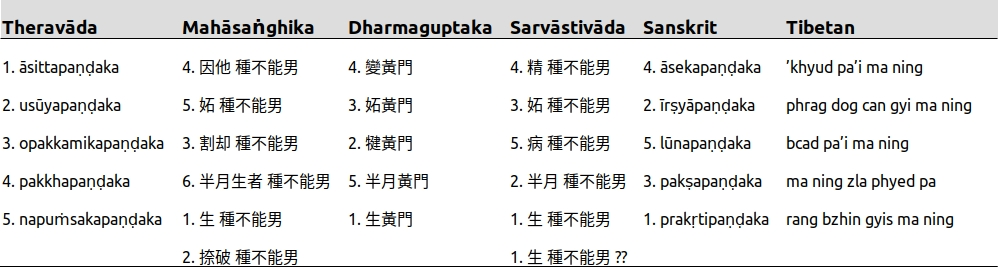
\includegraphics[width=\textwidth]{pandaka.jpg}
  \end{subfigure}
  \captionof{table}{The types of \textit{paṇḍaka} in the various schools.}
  \label{pandaka}
\end{figure}

It is striking that the \textit{Dharmaguptaka} \textit{Vinaya} continues to describe several types of castrated men but does not equate these to the term \textit{paṇḍaka}, while the word used for \textit{paṇḍaka} is 黃門 (i.e. `eunuch'), which is the exact definition of a castrated man.

The \textit{Theravāda} and \textit{Mahīśāsaka} \textit{Vinayas} agree on the background story and do not mention a list of types of \textit{paṇḍakas}, but the five types of \textit{paṇḍakas} are described in the commentaries. The other \textit{Vinayas} all have a list of \textit{paṇḍakas} who are not allowed to ordain but some of these types differ from each other or seem to have a different description. Bhikkhu Sujato\footnote{\cite{sujato2009} pages 216–217.} also observes that there are various terms where ``... a statement on the matter is found explicitly in all or most of the mainland \textit{Vinayas}, while the Pali Canon is silent, and the judgment is found in the commentary.'' He therefore concludes that there is an obvious explanation for this pattern, namely that the Pali is earlier. This is also confirmed by Zwilling and Sweet who write: ``... both Pali and Sanskrit Buddhism accepted a list of five kinds of \textit{paṇḍakas}, all of which are known to the brahminical and Jain traditions as varieties of \textit{ṣaṇḍas} and \textit{napuṁsakas}; this list seems an obvious later scholastic accretion.''\footnote{\cite{zwilling2000} page 117.}

It is therefore likely that at the time when the five types of \textit{paṇḍakas} were introduced, the \textit{Theravāda} and \textit{Mahīśāsaka} \textit{Vinayas} were already closed and therefore these five types appear in the commentarial text instead.\footnote{Although the \textit{Samantapāsādikā} is attributed to Buddhaghosa in the 5\textsuperscript{th} Century CE, this was based on earlier commentaries, now lost, in Prakrit and Sinhala, which were written down at the same time as the Canon, in the last Century BCE. As we see here, some material in the commentaries is found in canonical texts of other schools, suggesting an early common source.} 

The fact that the descriptions of the five terms do not always seem to match seamlessly between schools and that there are conflicting descriptions of a castrated man in the \textit{Dharmaguptaka} and \textit{Mahīśāsaka} \textit{Vinayas} seems to point to some ambiguity as to the meaning of the term \textit{paṇḍaka}; it seems that the Chinese scribes were unsure about the exact meaning.

In Appendix \ref{appendix2}, \ref{chinese1}, I have charted the various terms as they appear in the Chinese \textit{Taishō Tripiṭaka}. Both terms that denote \textit{paṇḍaka} are most prominent in the \textit{Vinaya} collections and are also present in the later \textit{Abhidhamma} and commentaries. This follows the same pattern as we have seen in the Pali and Sanskrit charts. The Tibetan charts in Figure \ref{tibetan1} also show this pattern.

\subsection{Development of the Paṇḍaka in the Scriptures}
After having looked at the references and descriptions of the word \textit{paṇḍaka} in Vedic texts, Jain discussions and Buddhist scriptures in both Pali and Chinese, a clearer picture emerges of what the \textit{paṇḍaka} really is and the reasons behind the Buddhist rules against ordination.

As we have seen in the previous chapter the oldest occurrence of the terms \textit{paṇḍaka} and \textit{klība} as sub-categories of the \textit{napuṁsaka} (`neither male nor female') happened just after the late Vedic period. They are the `not males', the `impotent', destined to play a role in the larger fabric of Indian religion, society and culture. They are the embodiment of the feminine in the masculine, a living myth. They are categorised by their feminine behavior and dress, their impotence, and their occupation as religious dancers and singers. They are there to remind us of the deeply ambivalent attitude of men towards women and women's sexuality; their desire for, and at the same time their fear of the feminine. Allan \cite{bomhard} points out that the word can be a loan-word from the Dravidian \textit{peṇṭan, peṇṭakan, peṇṭakam}, which can mean both hermaphrodite and eunuch. This is interesting because it is clear that at least in Dravidian no difference is made between a eunuch and a hermaphrodite and I believe that the way we need to see the term \textit{paṇḍaka} is indeed as embodying aspects of both these terms.

As none of the words \textit{paṇḍaka}, \textit{klība} and \textit{napuṁsaka} appear in the early Buddhist \textit{Suttas} or early parts of the \textit{Vinaya} and seem out of place in the Buddhist scriptures in the light of the Dhamma taught in the overall Canon but are found elsewhere in Jain or other Indic texts, there is a fair chance that these rules in the \textit{Vinaya} do not originate from the Buddha himself. Most likely the word \textit{paṇḍaka} entered the \textit{Vinaya} as part of the redaction during the Second Council, especially since we have seen that this redaction occurred at a time when a wider religious debate with regards to the position of women in religious life was taking place.\footnote{\cite{sujato2009} pages 141–142 and 215–216.} As this discussion hinged on what it means to be a `male' or `female', as a consequence what it means to be `neither male nor female' was discussed also. The \textit{Vinaya} describes the \textit{paṇḍaka} as hyperlibidinous and unable to maintain his monastic precepts, which is an idea also found in the Jain texts where it is explained as the result of him possessing both male and female \textit{veda}. But the \textit{Vinaya} itself falls short of defining a \textit{paṇḍaka} as anything else than simply hyperlibidinous and no further explanations are offered. 

\begin{figure}[!htbp]
  \begin{subfigure}{0.45\textwidth}
    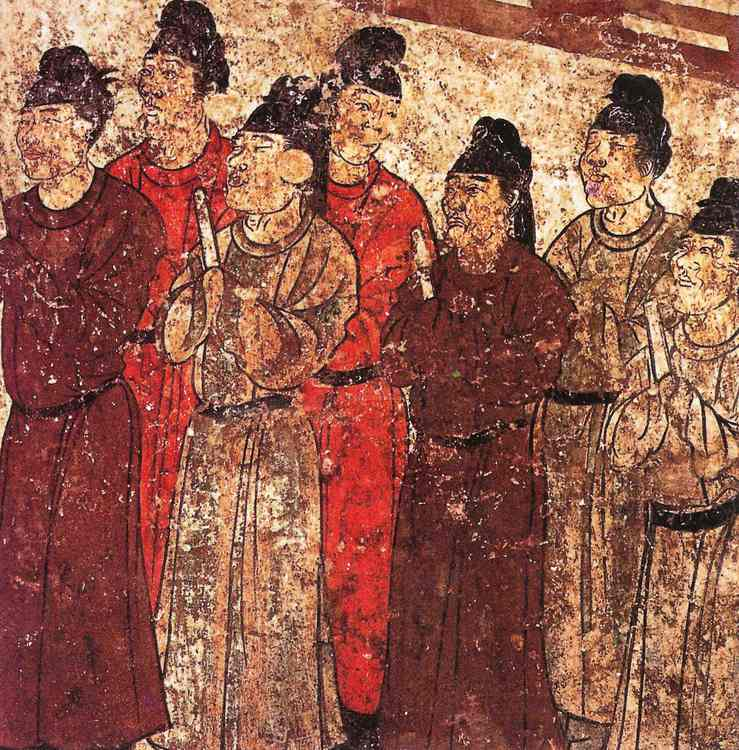
\includegraphics[width=\textwidth]{Eunuchs-in-ancient-China.jpg}
    \caption{Palace eunuchs in ancient China}
  \end{subfigure}
  \hfill
  \begin{subfigure}{0.45\textwidth}
    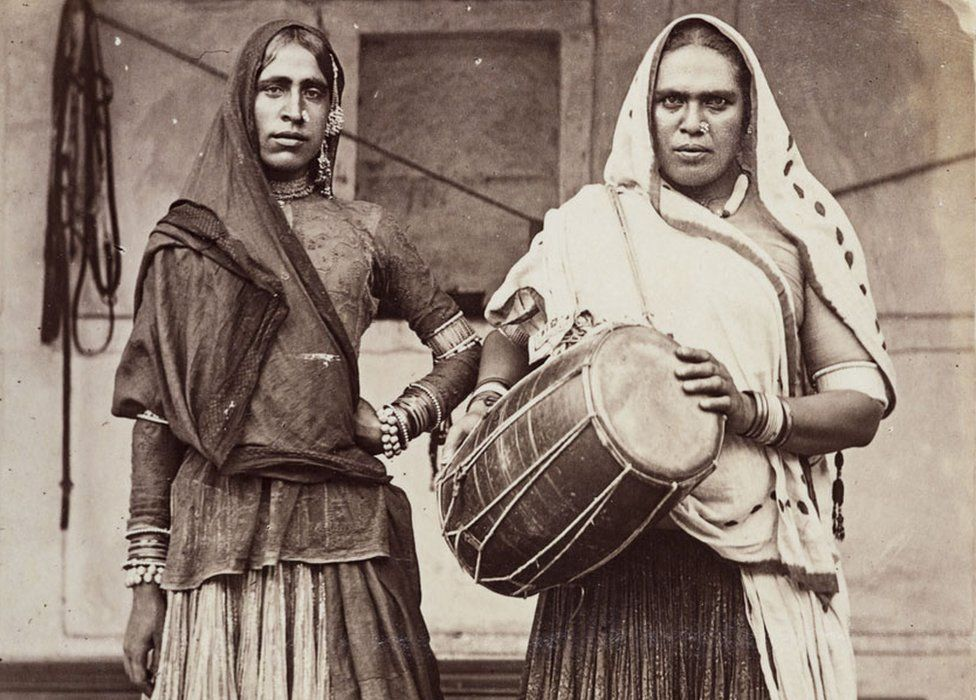
\includegraphics[width=\textwidth]{hijra.jpg}
    \caption{Hijra in India}
  \end{subfigure}
\setcounter{figure}{0}
\captionof{figure}{}
\label{eunuchs}
\end{figure}

It is in the later commentaries that we find more of a description in the form of the five types of \textit{paṇḍakas}. But this also causes further confusion because the concept in its entirety did not seem to be known to the translators of the Chinese texts so they used words they knew from their own culture. There the word \textit{paṇḍaka} was first translated as `impotent' (不能男) and later as `eunuch' (黃門). The translation `eunuch' however was taken from the words `yellow gate', denoting the Han Dynasty imperial palace eunuchs. This was possibly the only way that the Chinese could relate to a \textit{paṇḍaka}, being unfamiliar with the rich religious concept that they embody. It is clear that the Chinese palace eunuchs cannot be compared to the \textit{hijras} from India, who are most likely the closest modern-day representative of what the \textit{paṇḍakas} would have been (see Figure \ref{eunuchs}).

The concept of \textit{paṇḍaka} does not allow itself to be reduced to a mere word to make it acceptable and understandable for the rational mind. The people this term referred to showed a combination of sex- and gender-characteristics and had a religious (and probably sexual) role in society. They are the divine representation of the feminine within the masculine. It is the human representation of the mythical tales which have deep psychological roots, namely the ambivalence that leads to the inner struggle between man's love of the feminine and his fear thereof. The concept of \textit{paṇḍaka} does not match any contemporary notions. Both the \textit{paṇḍaka} and the 黃門 only have meaning in the unique social context in which these terms existed and cannot be reduced to their emasculated body nor to any other bodily characteristic.
